\chapter{First Step with Portenta Vision Shield}

The Arduino Portenta Vision Shield is an addon board providing machine vision capabilities and additional connectivity to the Portenta family of Arduino boards, designed to meet the needs of industrial automations. The Portenta Vision Shield connects via a high density connector to the Portenta H7 with minimal hardware and software setup.

\begin{figure}
	\begin{center}
		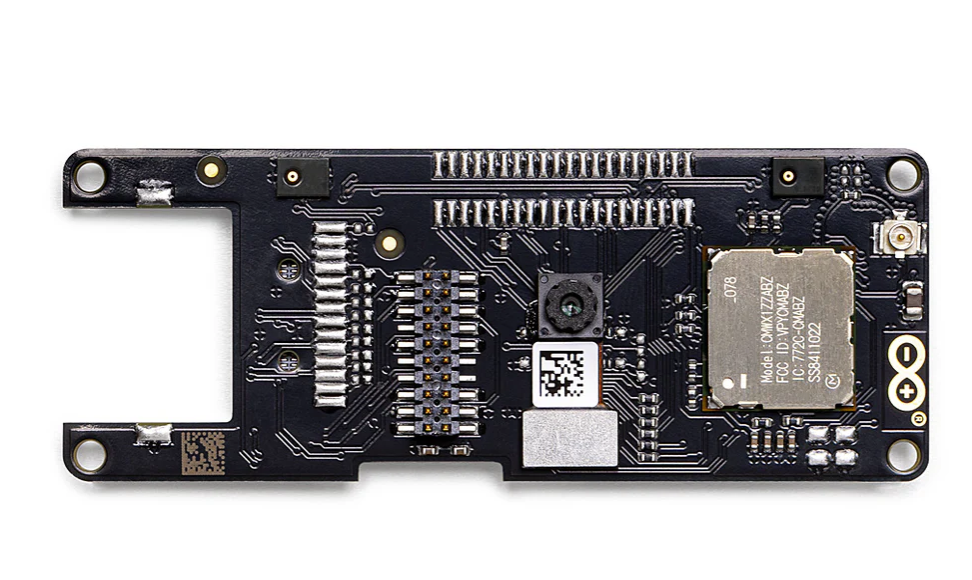
\includegraphics[width=0.7\linewidth]{Images/VisionShield/VisionShield.png}
		\caption{VisionShield}
		\label{VisionShield}
	\end{center}
\end{figure}

\section{Introduction}
In this chapter we will be going through the steps required for connecting the 
Arduino Portenta H7 with the Vision Shield using the OpenMV IDE and processing sketch.
Further, we will be looking at the overview of the OpenMV IDE
and what are the tools provided in the IDE. Finally, we will be implementing some of
the example programs provided in the OpenMV IDE. \cite{portentaH7visionshield:2024}

\section{Getting Started With the Portenta Vision Shield Camera}
This example shows you how to capture frames from the Arduino Portenta Vision Shield Camera module and visualize the video output through a Processing sketch, refer figure ~\ref{VisionShield} \cite{portentaVisionShieldCamera:2024}

\subsection{Required Hardware and Software:}
\begin{itemize}
	\item Portenta H7
	\item Portenta Vision Shield (LoRa or Ethernet)
	\item USB-C cable
	\item Arduino IDE 2.3.2
	\item Processing software \cite{portentaVisionShieldCamera:2024}
\end{itemize}
\subsection{Instructions:}
Accessing the Portenta Vision Shield's camera data is done with the help of both Arduino and the Processing IDE. The Arduino sketch handles the capture of image data by the on-board camera, while the java applet created with Processing helps to visualize this data with the help of a serial connection. The following steps will run you through how to capture, package the data through the serial port and visualize the output in Processing. \cite{portentaVisionShieldCamera:2024}

	\subsubsection{The Basic Setup:} Connect the Portenta Vision Shield to your Portenta H7 as shown in the figure ~\ref{Connection VS}. The top and bottom high density connecters are connected to the corresponding ones on the underside of the H7 board. Plug in the H7 to your computer using the USB-C cable. \cite{portentaVisionShieldCamera:2024}
	\begin{figure}
		\begin{center}
			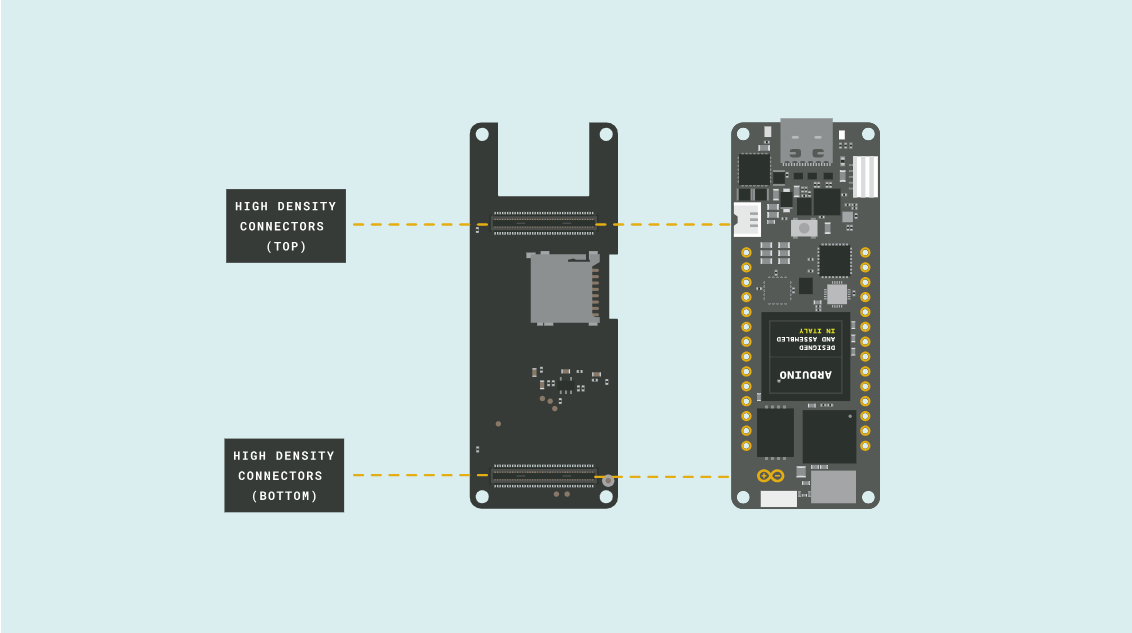
\includegraphics[width=0.7\linewidth]{Images/VisionShield/Connection VS.png}
			\caption{Connection VS}
			\label{Connection VS}
		\end{center}
	\end{figure}
	\newline
	Open the board manager in the Arduino IDE and install the latest version of the Portenta Core which is v4.1.5 as shown in the figure ~\ref{Portentaport}.
	
	\begin{figure}
		\begin{center}
			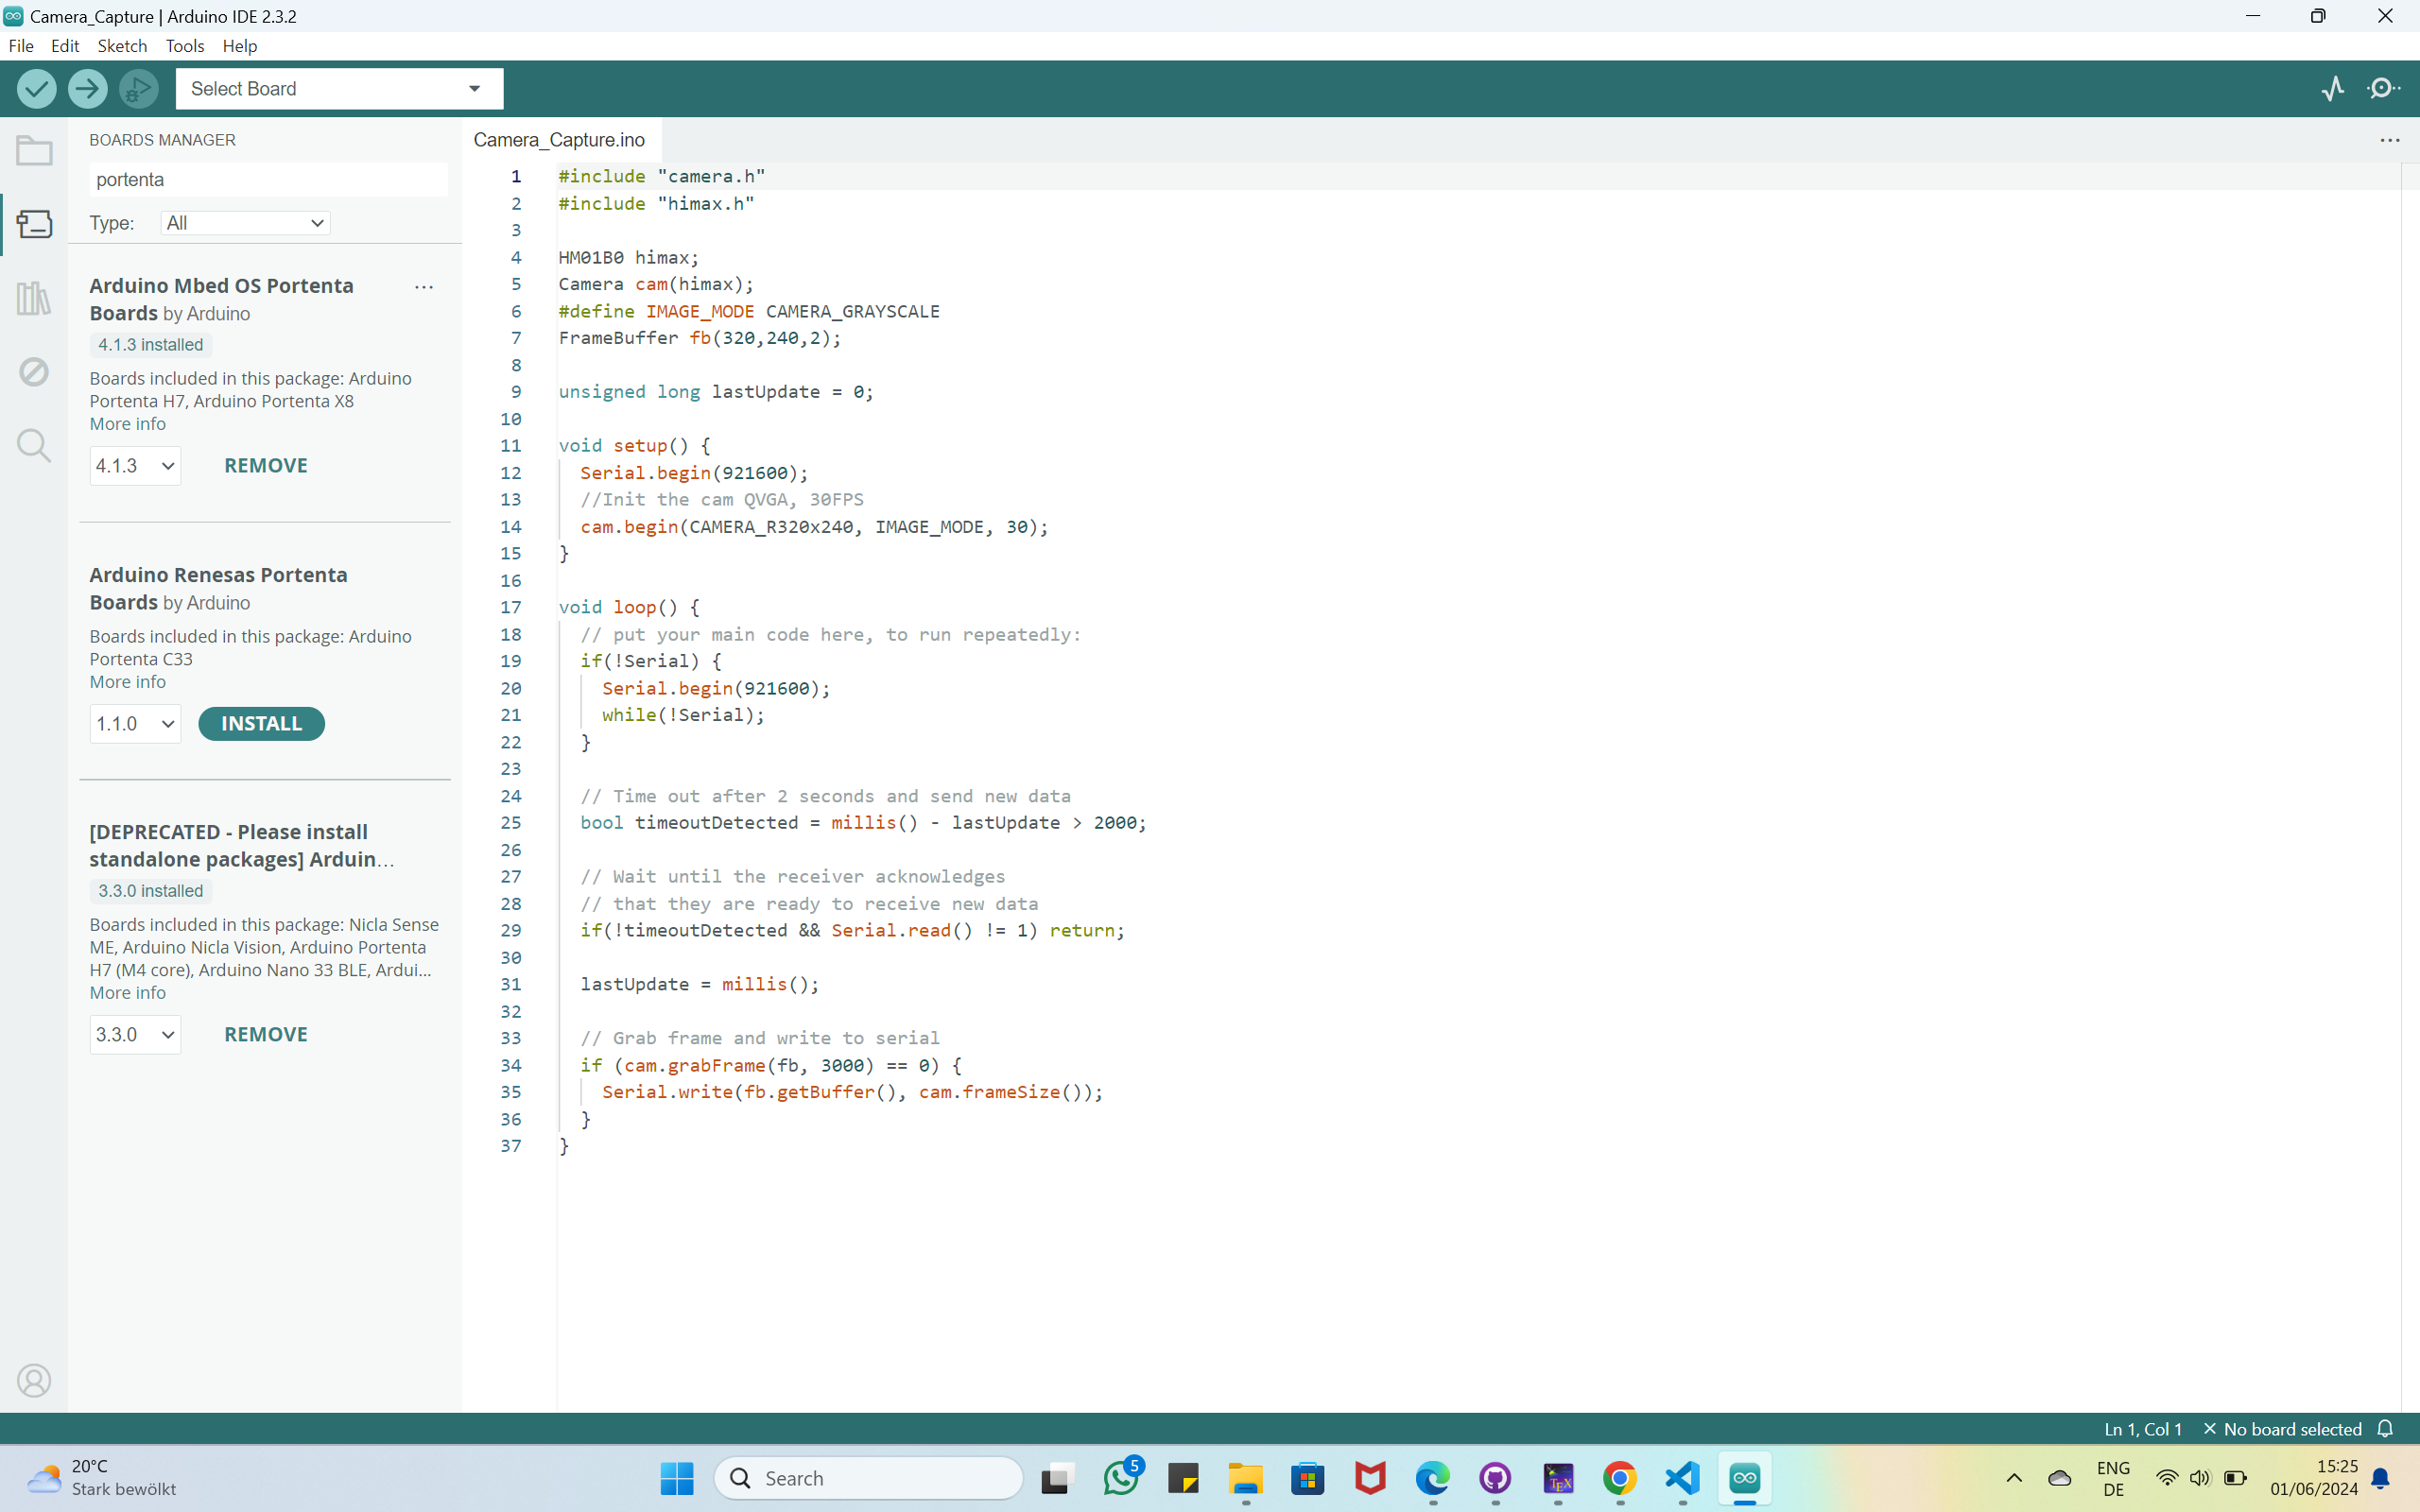
\includegraphics[width=0.7\linewidth]{Images/PortentaH7/Portentaport.png}
			\caption{Portentaport}
			\label{Portentaport}
		\end{center}
	\end{figure}
	
	\subsubsection{Capturing the Frames:} Create a new Arduino sketch called \SHELL{CameraCaptureRawBytes.ino}
	
	To capture the frames you will need to use the functions contained in \SHELL{camera.h} which comes with the Portenta core. This library contains all APIs related to frame capturing, motion detection and pattern recognition. Include the header file in your sketch.
	
	
	\begin{lstlisting}[language=C++, frame=single, numbers=left, basicstyle=\ttfamily\small]
		#include "camera.h"
		#include "himax.h"
	\end{lstlisting}
	Next, let's initialize a camera object and a frame buffer of the size \SHELL{320*240 (76'800 bytes).}
	
	\begin{lstlisting}[language=C++, frame=single, numbers=left, basicstyle=\ttfamily\small]
		HM01B0 himax;
		Camera cam(himax);
		#define IMAGE_MODE CAMERA_GRAYSCALE
		FrameBuffer fb(320,240,2);
		unsigned long lastUpdate = 0;
	\end{lstlisting}
	
	In the \SHELL{setup()} function, let's start the Serial communication at \SHELL{921600 baud rate} and initialize the camera using \SHELL{cam.begin()}.
	
	\begin{lstlisting}[language=C++, frame=single, numbers=left, basicstyle=\ttfamily\small]
		void setup() {
			Serial.begin(921600);
			//Init the cam QVGA, 30FPS
			cam.begin(CAMERA_R320x240, IMAGE_MODE, 30);
		}
	\end{lstlisting}
	In the loop you need to capture each Frame and send it over a serial connection to the Processing sketch that will display the frames. You will use the function to fetch the frame from the frame buffer and save it into your custom data buffer.
	
	\begin{lstlisting}[language=C++, frame=single, numbers=left, basicstyle=\ttfamily\small]
		void loop() {
			// put your main code here, to run repeatedly:
			if(!Serial) {    
				Serial.begin(921600);
				while(!Serial);
			}
			
			// Time out after 2 seconds and send new data
			bool timeoutDetected = millis() - lastUpdate > 2000;
			
			// Wait until the receiver acknowledges
			// that they are ready to receive new data
			if(!timeoutDetected && Serial.read() != 1) return;
			
			lastUpdate = millis();
			
			// Grab frame and write to serial
			if (cam.grabFrame(fb, 3000) == 0) {
				Serial.write(fb.getBuffer(), cam.frameSize());
			}
		}
	\end{lstlisting}
	
	\subsubsection{Create the Processing Sketch:} Open a new processing sketch file and name it CameraCapture.pde. ~\ref{Processingimage} \cite{portentaVisionShieldCamera:2024}
	
	\begin{figure}
		\begin{center}
			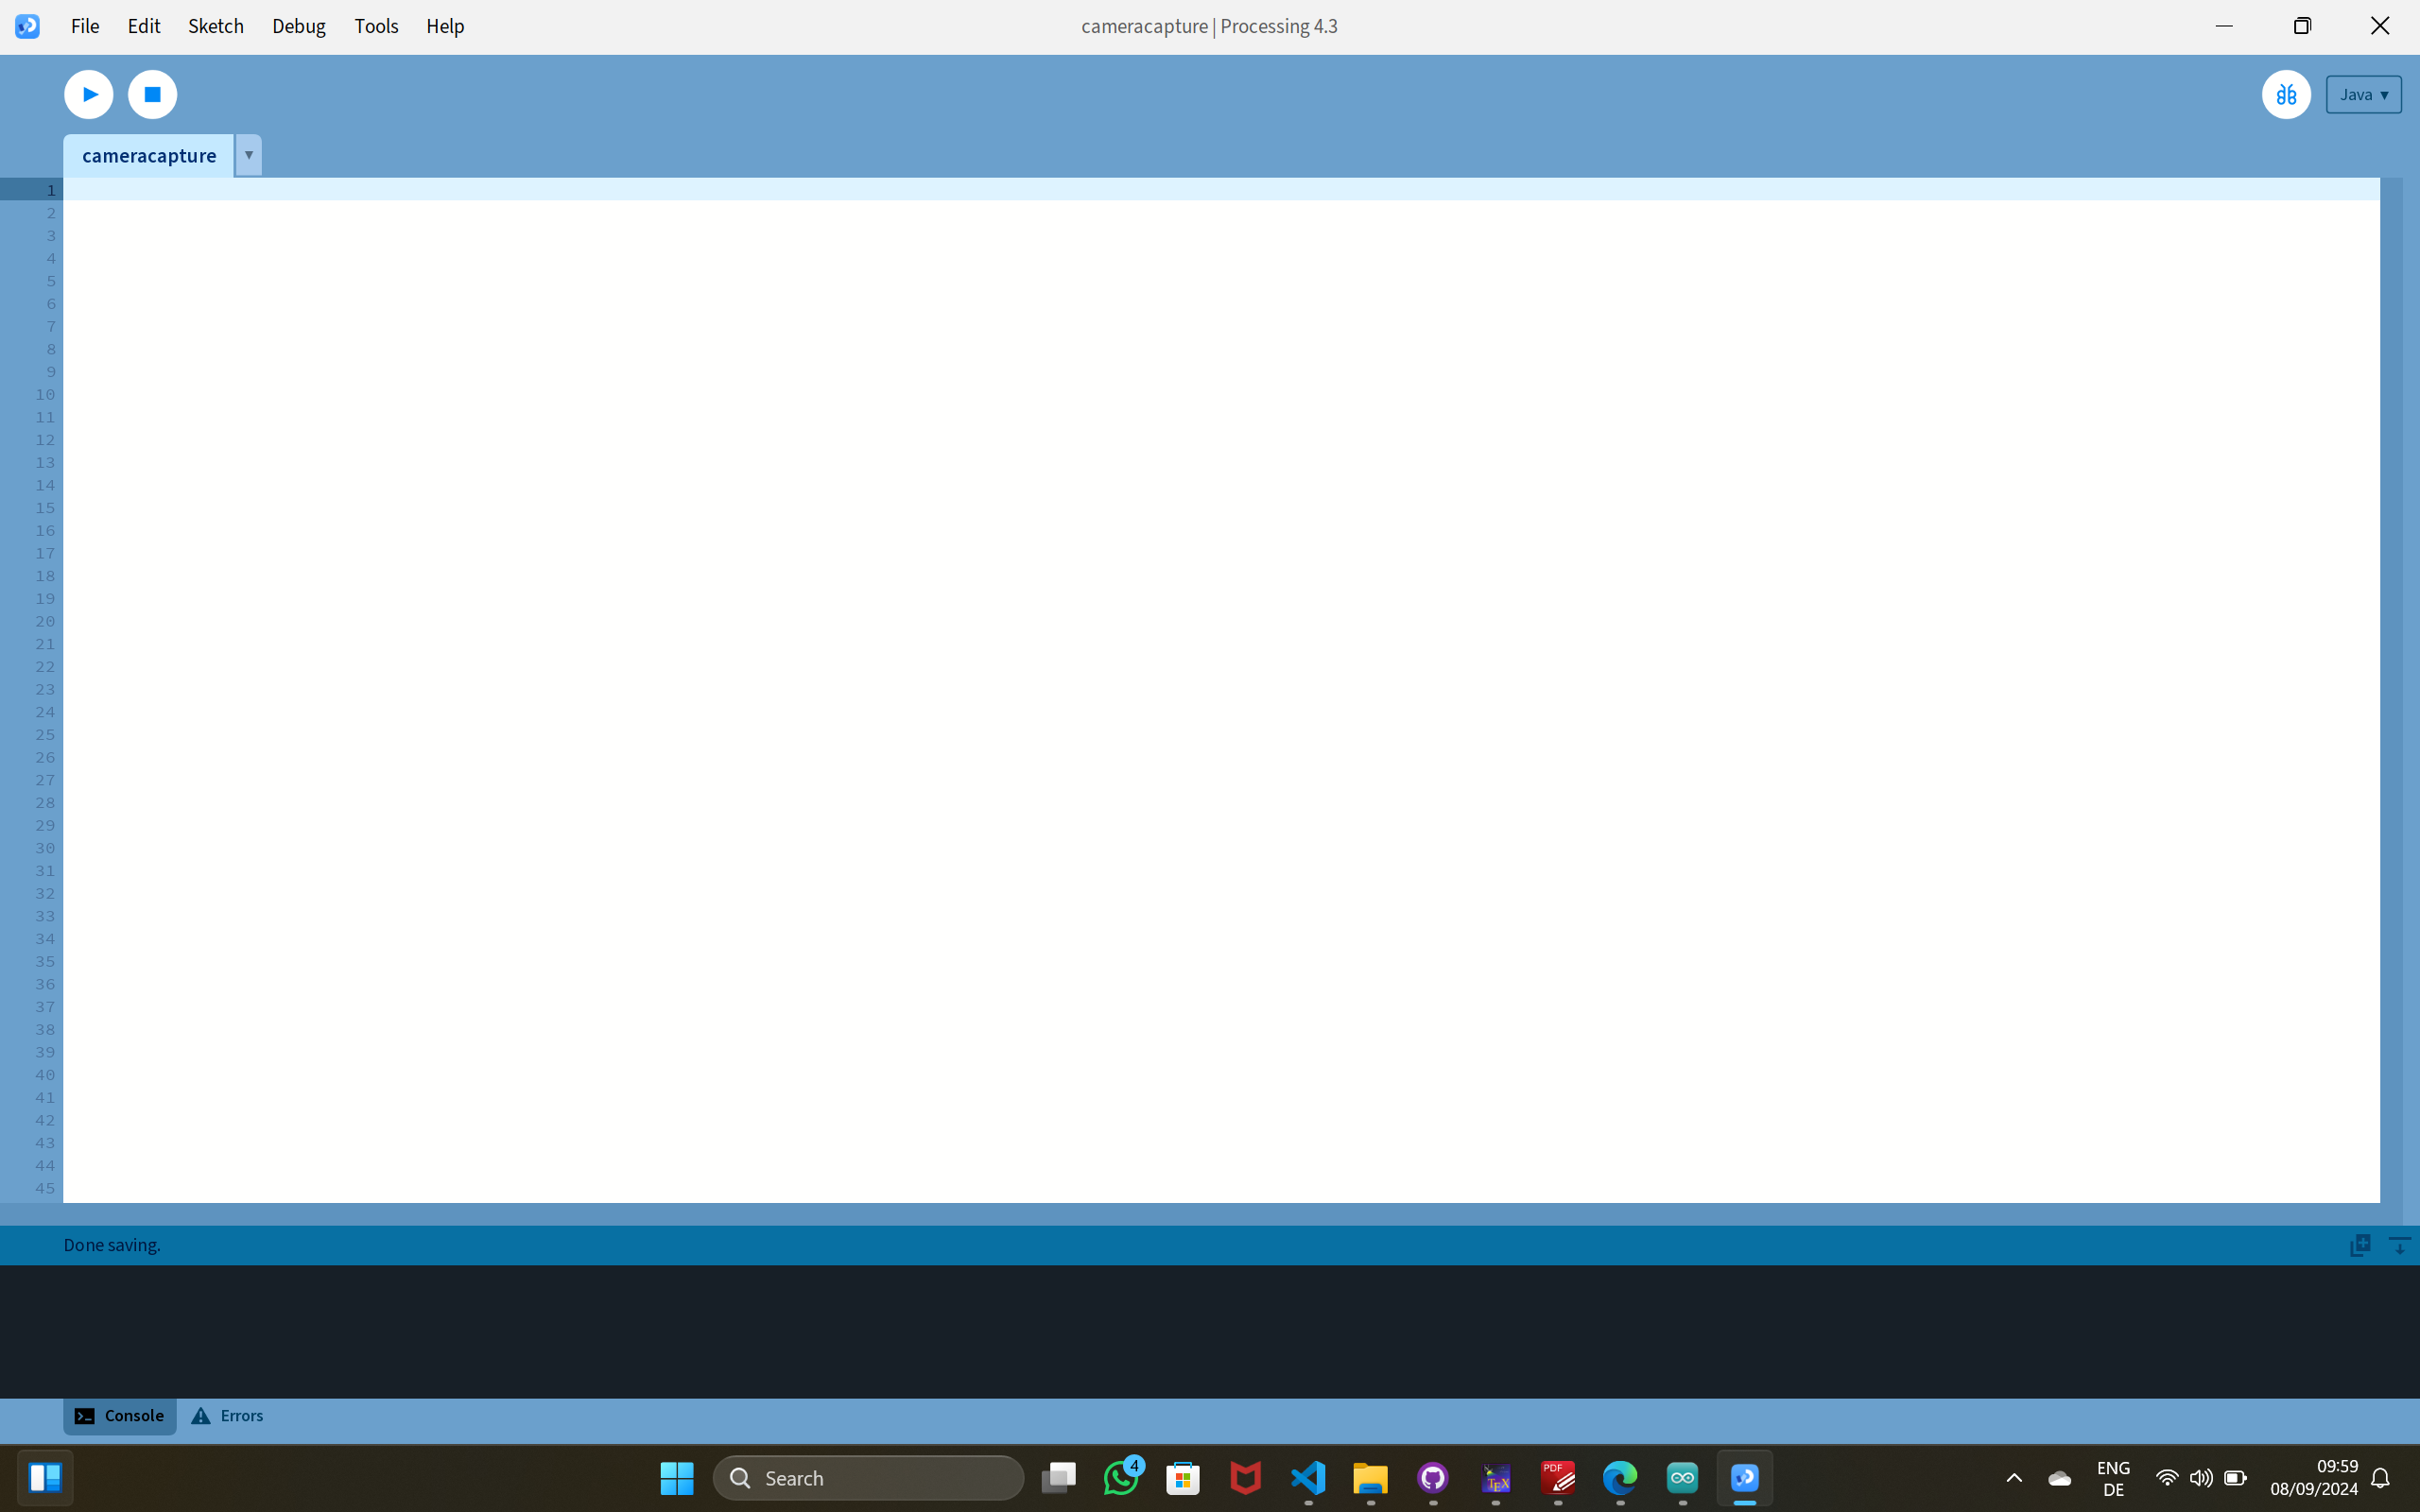
\includegraphics[width=0.7\linewidth]{Images/VisionShield/CameracaptureProcessing.png}
			\caption{Processingimage}
			\label{Processingimage}
		\end{center}
	\end{figure}
	
	Let's start by importing the libraries and initializing the variables you will need to process. To process the data sent by the Portenta Vision Shield, you will need to import the following libraries:
	
	\begin{enumerate}
		\item \SHELL{processing.serial.*:} a Serial Library that is used to read and write data to external devices over the serial line.
		\item \SHELL{java.nio.ByteBuffer:} a java class that provides access to operations on byte buffers
	\end{enumerate}
	
	\begin{lstlisting}[language=C++, frame=single, numbers=left, basicstyle=\ttfamily\small]
		import processing.serial.*;
		import java.nio.ByteBuffer;
	\end{lstlisting}
	Next, you can initialize the following variables to process the received pixels from the serial port. You can set the dimensions, pixel count and bytes required per frame.
	
	\begin{lstlisting}[language=C++, frame=single, numbers=left, basicstyle=\ttfamily\small]
		// must match resolution used in the sketch
		final int cameraWidth = 320;
		final int cameraHeight = 240;
		final int cameraBytesPerPixel = 1;
		final int cameraPixelCount = cameraWidth * cameraHeight;
		final int bytesPerFrame = cameraWidth * cameraHeight * cameraBytesPerPixel;
	\end{lstlisting}
	
	To receive the frames, you will need a Serial port, a PImage object and an array to store the pixel values of the frame. Add the following variables to the code.
		
	\begin{lstlisting}[language=C++, frame=single, numbers=left, basicstyle=\ttfamily\small]
		Serial myPort;
		PImage myImage;
		byte[] frameBuffer = new byte[bytesPerFrame];
		int pixelPosition = 0;
		int lastUpdate = 0;
		boolean shouldRedraw = false;
	\end{lstlisting}
	Here, you will establish a connection to the serial port and prepare the buffer to store the frame pixels. Additionally, you can send a byte to the Arduino sketch from Processing to let it know that it is ready to receive data.
	
	\begin{lstlisting}[language=C++, frame=single, numbers=left, basicstyle=\ttfamily\small]
		void setup() {
			size(640, 480);
			
			// if you know the serial port name
			//myPort = new Serial(this, "COM5", 921600);                  // Windows
			//myPort = new Serial(this, "/dev/ttyACM0", 921600);          // Linux
			myPort = new Serial(this, "/dev/cu.usbmodem14101", 921600);   // Mac
			
			// Set the number of bytes to buffer 
			myPort.buffer(bytesPerFrame)
			
			// Create an image based on the camera's dimensions and format
			myImage = createImage(cameraWidth, cameraHeight, ALPHA);
			
			// Let the Arduino sketch know we're ready to receive data
			myPort.write(1);
		}
	\end{lstlisting}
	
	The draw function checks if the connection is still alive and if there is any new data that can be drawn as an image. In that case, the original image gets copied into a new image object so that it can be scaled up.
	
	\begin{lstlisting}[language=C++, frame=single, numbers=left, basicstyle=\ttfamily\small]
		void draw() {
			// Time out after 1.5 seconds and ask for new data
			if(millis() - lastUpdate > 1500) {
				println("Connection timed out.");
				myPort.clear();
				myPort.write(1);
			}
			
			if(shouldRedraw){    
				PImage img = myImage.copy();
				img.resize(640, 480);
				image(img, 0, 0);
				shouldRedraw = false;
			}
		}
	\end{lstlisting}
	
	\subsubsection{Visualizing the Frames:} For this step, you will use the \SHELL{serialEvent()} callback function to update the \SHELL{myImage} when a new data is received on the serial port.  \cite{portentaVisionShieldCamera:2024}
	
	\begin{lstlisting}[language=C++, frame=single, numbers=left, basicstyle=\ttfamily\small]
		void serialEvent(Serial myPort) {
			lastUpdate = millis();
			
			// read the received bytes
			myPort.readBytes(frameBuffer);
			
			// Access raw bytes via byte buffer  
			ByteBuffer bb = ByteBuffer.wrap(frameBuffer);
			
			int i = 0;
			
			while (bb.hasRemaining()) {
				// read 8-bit pixel
				byte pixelValue = bb.get();
				
				// set pixel color
				myImage.pixels[i++] = color(Byte.toUnsignedInt(pixelValue));    
			}
			
			myImage.updatePixels();
			
			// Ensures that the new image data is drawn in the next draw loop
			shouldRedraw = true;
			
			// Let the Arduino sketch know we received all pixels
			// and are ready for the next frame
			myPort.write(1);
		}
	\end{lstlisting}
	
	The first thing you can do inside this method is to update the timestamp when the last data was read. This is to detect and recover from a connection timeout. Then read the bytes from the frameBuffer array which you can do with the help of the \SHELL{readBytes()} method that returns the number of bytes read.
	
	\begin{lstlisting}[language=C++, frame=single, numbers=left, basicstyle=\ttfamily\small]
		lastUpdate = millis();
		
		// read the received bytes
		myPort.readBytes(frameBuffer);
	\end{lstlisting}
	
	Then the frame buffer is translated into a ByteBuffer that allows for easy and safe access to the underlying bytes without having to worry about the array indices.
	
	\begin{lstlisting}[language=C++, frame=single, numbers=left, basicstyle=\ttfamily\small]
		// Access raw bytes via byte buffer  
		ByteBuffer bb = ByteBuffer.wrap(frameBuffer);
	\end{lstlisting}
	Next we read the frame buffer and convert the bytes into pixel color values. The image gets constructed by sequentially filling the pixels array of the image. The conversion of the raw data is done with \SHELL{color()} and \SHELL{Byte.toUnsignedInt().}
	
	\begin{lstlisting}[language=C++, frame=single, numbers=left, basicstyle=\ttfamily\small]
		int i = 0;
		
		while (bb.hasRemaining()) {
			// read 8-bit pixel
			byte pixelValue = bb.get();
			
			// set pixel color
			myImage.pixels[i++] = color(Byte.toUnsignedInt(pixelValue));    
		}
	\end{lstlisting}
	
	Once all the pixels have been updated, you need to tell the sketch to redraw the image. Additionally, you can send an acknowledgement back to the arduino sketch to ask it to send the pixels for the next frame. You can update the image with \SHELL{updatePixels()} and write \SHELL{1} to the serial port for the acknowledgement.
	
	\begin{lstlisting}[language=C++, frame=single, numbers=left, basicstyle=\ttfamily\small]
		myImage.updatePixels();
		
		// Ensures that the new image data is drawn in the next draw loop
		shouldRedraw = true;
		
		// Let the Arduino sketch know we received all pixels
		// and are ready for the next frame
		myPort.write(1);
	\end{lstlisting}
	
	\subsubsection{Upload the Sketch:} Select the right serial port on your IDE and upload the Arduino sketch to your Portenta H7. After a successful upload, run the \SHELL{CameraViewer.pde} sketch in Processing. You should be able to see the rendered camera output on the Processing canvas. ~\ref{CameraOutput} \cite{portentaVisionShieldCamera:2024}
	
	\begin{figure}
		\begin{center}
			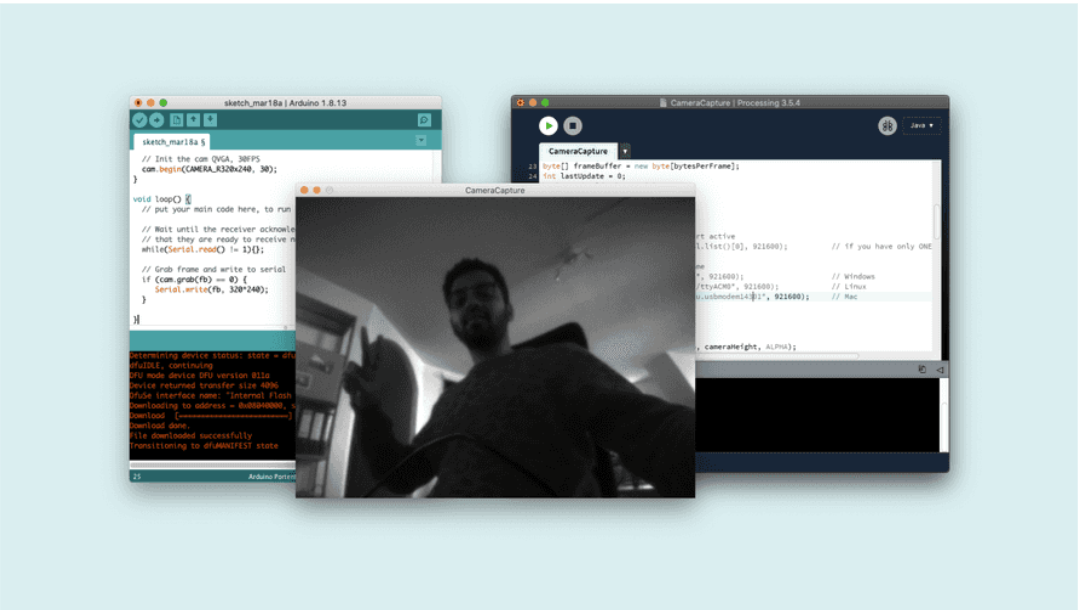
\includegraphics[width=0.7\linewidth]{Images/VisionShield/CameraOutput.png}
			\caption{CameraOutput}
			\label{CameraOutput}
		\end{center}
	\end{figure}
	
\subsection{Conclusion:}
	In this example you learnt how to capture the frames from your Portenta Vision Shield's Camera and to visualize the frames through Processing. This knowledge can be useful for you to build and experiment simple computer vision applications for both outdoor and indoor environments.
	
	\subsubsection{Complete Sketch:}
	The \SHELL{CaptureRawBytes.ino} Sketch. ~\ref{CaptureRawBytes}
	
		{
			\captionof{code}{Simple sketch to capture the image from vision shield}\label{CaptureRawBytes}
			\ArduinoExternal{}{../Code/Vision shield/Camera Capture/CaptureRawBytes.ino}
		}
	
		
	The \SHELL{CameraViewer.pde} Sketch. ~\ref{cameraviewer}
		
		{
			\captionof{code}{Simple sketch to capture the image from vision shield}\label{cameraviewer}
			\ArduinoExternal{}{../Code/Vision shield/Camera Capture/cameraviewer.pde}
		}





\section{Saving Bitmap Camera Images to the SD Card and PC}
This tutorial shows you how to capture a frame from the Portenta Vision Shield Camera module and save the output as a bitmap image. It will allow you to see the output directly on your computer without using any third party tool. ~\ref{VisionShield} \cite{portentaCameraToBitmap:2024}

\begin{figure}
	\begin{center}
		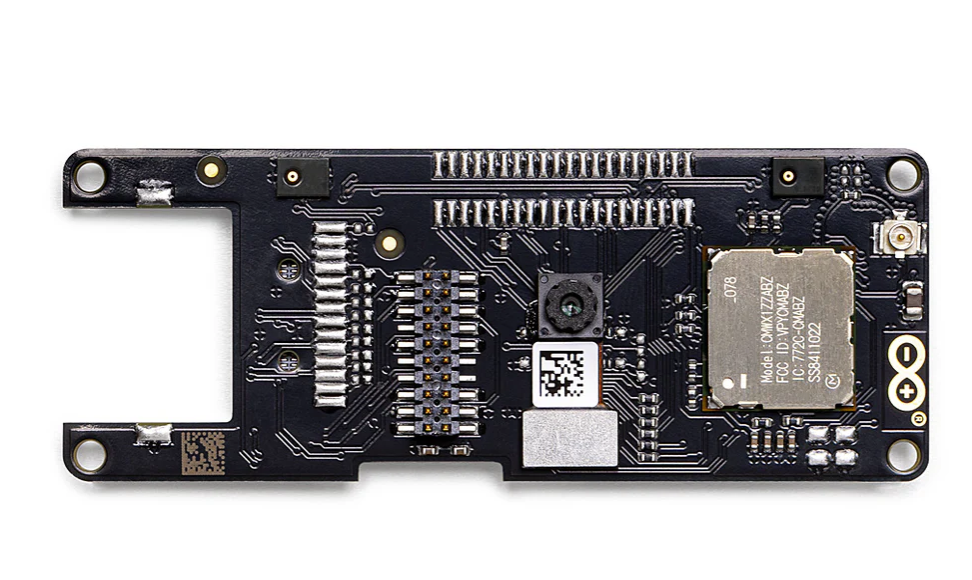
\includegraphics[width=0.7\linewidth]{Images/VisionShield/VisionShield.png}
		\caption{VisionShield}
		\label{VisionShield}
	\end{center}
\end{figure}

\subsection{Goals:}
\begin{itemize}
	\item Capturing a frame from the camera.
	\item Make the bitmap binary file with the correct settings.
	\item Save the bitmap on an SD Card.
	\item Save the bitmap on an PC: 
	\item Visualize the captured image on your computer. \cite{portentaCameraToBitmap:2024}
\end{itemize}

\subsection{Required Hardware and Software:}
\begin{itemize}
	\item Portenta H7
	\item Portenta Vision Shield (LoRa or Ethernet)
	\item USB-C cable
	\item Micro SD card
	\item Arduino IDE \cite{portentaCameraToBitmap:2024}
\end{itemize}

\subsection{Instructions:}

\subsubsection{The Setup:} Connect the Portenta Vision Shield to your Portenta H7 as shown in the figure. The top and bottom high density connectors are connected to the corresponding ones on the underside of the H7 board. Plug in the H7 to your computer using the USB-C cable. \cite{portentaCameraToBitmap:2024}

\begin{figure}
	\begin{center}
		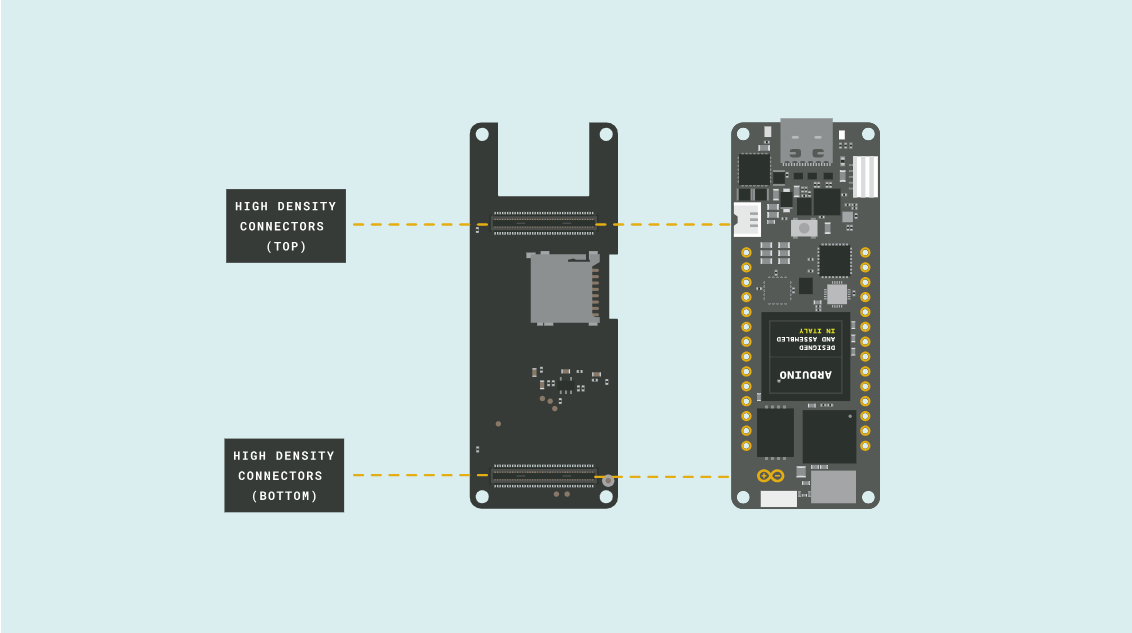
\includegraphics[width=0.7\linewidth]{Images/VisionShield/Connection VS.png}
		\caption{Connection Vision Shield}
		\label{Connection VS}
	\end{center}
\end{figure}

\textbf{The Camera}
\newline
You will be using the \SHELL{Himax HM-01B0} camera module which has a resolution of 320 by 240 and the output data its in grayscale with 8 bits per pixel (bpp). It is important to have this in mind as the \SHELL{.bmp} (bitmap) format has some needed configuration depending on the data being used. \cite{portentaCameraToBitmap:2024}
\newline


\begin{lstlisting}[language=C++, frame=single, numbers=left, basicstyle=\ttfamily\small]
	#include "camera.h" // Multi Media Card APIs
	#include "himax.h"  // API to read from the Himax camera found on the Portenta Vision Shield
\end{lstlisting}

\textbf{Bitmap File Format}\newline
The bitmap binary file needs to contain some information in order to tell the computer for example the resolution of the picture and the bit-depth (bpp). Bit depth refers to the color information stored in the image. The higher the bit depth of an image, the more colors it can store. As the bit depth increases, the file size of the image also increases, because more color information has to be stored for each pixel in the image.

The following table ~\ref{tab:bitmap} shows all the headers, the size of its buffer, offsets, the settings that are being used with their details: \cite{portentaCameraToBitmap:2024}

\begin{table}[h]
	\centering
	\begin{tabular}{|l|l|p{8cm}|}
		\hline
		\textbf{Name} & \textbf{Size} & \textbf{Details} \\ \hline
		DIB & 14 Bytes & Bitmap information, setting the size of the file. \\ \hline
		File Header & 40 Bytes & This header requires the resolution and the bpp. \\ \hline
		Palette (Color Map) & 1025 Bytes & This header is mandatory on bitmaps with a bpp $\leq$ 8, setting the grayscale. \\ \hline
		Image data & 76800 Bytes & The raw image data, in this case, each pixel has 8 bits (1 Byte) and the resolution is 320 x 240, with no compression. \\ \hline
	\end{tabular}
	\caption{Description of the bitmap file structure.}
	\label{tab:bitmap}
\end{table}

The final size of the file is 77.879 KB.

\subsubsection{The Sketch:} You can find the sketch on the latest version of the Arduino Pro Tutorials at \SHELL{examples > Vision Shield to SD Card bmp > visionShieldBitmap.ino} 

First you need to include the needed libraries \cite{portentaCameraToBitmap:2024}

\begin{lstlisting}[language=C++, frame=single, numbers=left, basicstyle=\ttfamily\small]
	#include "SDMMCBlockDevice.h" // Multi Media Card APIs
	#include "FATFileSystem.h"    // Mbed API for portable  and embedded systems
	
	#include "camera.h" // Arduino Mbed Core Camera APIs
	#include "himax.h"  // API to read from the Himax camera found on the Portenta Vision Shield
\end{lstlisting}

Then define the following objects with their respective constructor blockDevice and fileSystem objects, needed for getting access to the SD Card and the file system. \cite{portentaCameraToBitmap:2024}

\begin{lstlisting}[language=C++, frame=single, numbers=left, basicstyle=\ttfamily\small]
	#include "SDMMCBlockDevice.h" // Multi Media Card APIs
	#include "FATFileSystem.h"    // API to run operations on a FAT file system
	SDMMCBlockDevice blockDevice;
	mbed FATFileSystem fileSystem("fs");
	
	#include "camera.h" // Arduino Mbed Core Camera APIs
	#include "himax.h"  // API to read from the Himax camera found on the Portenta Vision Shield
	HM01B0 himax;
	Camera cam(himax);
	
	FrameBuffer frameBuffer; // Buffer to save the camera stream
\end{lstlisting}

For the bitmap headers binary file you will need some information like the resolution of the image, the bits per pixel and more; so you can define your settings as shown: \cite{portentaCameraToBitmap:2024}

\begin{lstlisting}[language=C++, frame=single, numbers=left, basicstyle=\ttfamily\small]
	// Settings for our setup
	#define IMAGE_HEIGHT (unsigned int)240
	#define IMAGE_WIDTH (unsigned int)320
	#define IMAGE_MODE CAMERA_GRAYSCALE
	#define BITS_PER_PIXEL (unsigned int)8
	#define PALETTE_COLORS_AMOUNT (unsigned int)(pow(2, BITS_PER_PIXEL))
	#define PALETTE_SIZE  (unsigned int)(PALETTE_COLORS_AMOUNT * 4) // 4 bytes = 32bit per color (3 bytes RGB and 1 byte 0x00)
	#define IMAGE_PATH "/fs/image.bmp"
	
	// Headers info
	#define BITMAP_FILE_HEADER_SIZE (unsigned int)14 // For storing general information about the bitmap image file
	#define DIB_HEADER_SIZE (unsigned int)40 // For storing information about the image and define the pixel format
	#define HEADER_SIZE (BITMAP_FILE_HEADER_SIZE + DIB_HEADER_SIZE)
\end{lstlisting}

The program has the following functions declared: \cite{portentaCameraToBitmap:2024}
\begin{enumerate}
	\item \SHELL{void mountSDCard()}
	\item \SHELL{unsigned char * captureImage()}
	\item \SHELL{void setFileHeaders(bitmapFileHeaders, bitmapDIBHeader, fileSize)}
	\item \SHELL{void setColorMap(colorMap)}
	\item \SHELL{saveImage(imageData, imagePath)}
\end{enumerate}

To mount the SD Card you will use the following function in the sketch: \cite{portentaCameraToBitmap:2024}

\begin{lstlisting}[language=C++, frame=single, numbers=left, basicstyle=\ttfamily\small]
	// Mount File system block
	void mountSDCard(){
		int error = fileSystem.mount(blockDevice);
		if (error){
			Serial.println("Trying to reformat...");
			int formattingError = fileSystem.reformat(blockDevice);
			if (formattingError) {            
				Serial.println("No SD Card found");
				while (1);
			}
		}
	}
\end{lstlisting}

The function to capture the frame from the camera: \cite{portentaCameraToBitmap:2024}

\begin{lstlisting}[language=C++, frame=single, numbers=left, basicstyle=\ttfamily\small]
	// Get the raw image data (8bpp grayscale)
	unsigned char * captureImage(){
		if (cam.grabFrame(frameBuffer, 3000) == 0){
			return frameBuffer.getBuffer();
		} else {
			Serial.println("could not grab the frame");
			while (1);
		}
	}
\end{lstlisting}

To manipulate the file you will need to set the headers on the binary information as follows: \cite{portentaCameraToBitmap:2024}

\begin{lstlisting}[language=C++, frame=single, numbers=left, basicstyle=\ttfamily\small]
	// Set the headers data
	void setFileHeaders(unsigned char *bitmapFileHeader, unsigned char *bitmapDIBHeader, int fileSize){
		// Set the headers to 0
		memset(bitmapFileHeader, (unsigned char)(0), BITMAP_FILE_HEADER_SIZE);
		memset(bitmapDIBHeader, (unsigned char)(0), DIB_HEADER_SIZE);
		
		// File header
		bitmapFileHeader[0] = 'B';
		bitmapFileHeader[1] = 'M';
		bitmapFileHeader[2] = (unsigned char)(fileSize);
		bitmapFileHeader[3] = (unsigned char)(fileSize >> 8);
		bitmapFileHeader[4] = (unsigned char)(fileSize >> 16);
		bitmapFileHeader[5] = (unsigned char)(fileSize >> 24);
		bitmapFileHeader[10] = (unsigned char)HEADER_SIZE + PALETTE_SIZE;
		
		// Info header
		bitmapDIBHeader[0] = (unsigned char)(DIB_HEADER_SIZE);
		bitmapDIBHeader[4] = (unsigned char)(IMAGE_WIDTH);
		bitmapDIBHeader[5] = (unsigned char)(IMAGE_WIDTH >> 8);
		bitmapDIBHeader[8] = (unsigned char)(IMAGE_HEIGHT);
		bitmapDIBHeader[9] = (unsigned char)(IMAGE_HEIGHT >> 8);
		bitmapDIBHeader[14] = (unsigned char)(BITS_PER_PIXEL); }
\end{lstlisting}

In this case that our image (320x240) is 8 bits per pixel and grayscale on the bitmap rules you need to define the color table (color map) to assign an specific RGB color for our 8 bit color. On the following function it sets the color map as a grayscale of RGB colors from \SHELL{[R:0x00 G:0x00 B:0x00] to [R:0xFF G:0xFF B:0xFF]} \cite{portentaCameraToBitmap:2024}

The function in charge to save the image will use the previous functions to set the headers and write the buffers into the file \SHELL{image.bmp} \cite{portentaCameraToBitmap:2024}

\begin{lstlisting}[language=C++, frame=single, numbers=left, basicstyle=\ttfamily\small]
	// Save the headers and the image data into the .bmp file
	void saveImage(unsigned char *imageData, const char* imagePath){
		int fileSize = BITMAP_FILE_HEADER_SIZE + DIB_HEADER_SIZE + IMAGE_WIDTH * IMAGE_HEIGHT;
		FILE *file = fopen(imagePath, "w");
		
		// Bitmap structure (Head + DIB Head + ColorMap + binary image)
		unsigned char bitmapFileHeader[BITMAP_FILE_HEADER_SIZE];
		unsigned char bitmapDIBHeader[DIB_HEADER_SIZE];
		unsigned char colorMap[PALETTE_SIZE]; // Needed for < 8bpp grayscale bitmaps    
		
		setFileHeaders(bitmapFileHeader, bitmapDIBHeader, fileSize);
		setColorMap(colorMap);
		
		// Write the bitmap file
		fwrite(bitmapFileHeader, 1, BITMAP_FILE_HEADER_SIZE, file);
		fwrite(bitmapDIBHeader, 1, DIB_HEADER_SIZE, file);
		fwrite(colorMap, 1, PALETTE_SIZE, file);
		fwrite(imageData, 1, IMAGE_HEIGHT * IMAGE_WIDTH, file);
		
		// Close the file stream
		fclose(file);
	}
\end{lstlisting}

Then to have visual feedback lets add a blink function to make 3 blinks after the photo is taken, once the blue LED is ON it means the picture was taken. \cite{portentaCameraToBitmap:2024}

\begin{lstlisting}[language=C++, frame=single, numbers=left, basicstyle=\ttfamily\small]
	void countDownBlink(){
		for (int i = 0; i < 6; i++){
			digitalWrite(LEDG, i % 2);
			delay(500);
		}
		digitalWrite(LEDG, HIGH);
		digitalWrite(LEDB, LOW);
	}
\end{lstlisting}

Now that you have all the functions to be used, inside the \SHELL{setup()} its call them only once after the board restarts. \cite{portentaCameraToBitmap:2024}

\begin{lstlisting}[language=C++, frame=single, numbers=left, basicstyle=\ttfamily\small]
	void setup(){
		Serial.begin(115200);
		while (!Serial & millis() < 5000);
		
		Serial.println("Mounting SD Card...");
		mountSDCard();
		Serial.println("SD Card mounted.");
		
		// Init the cam QVGA, 30FPS, Grayscale
		if (!cam.begin(CAMERA_R320x240, IMAGE_MODE, 30)){
			Serial.println("Unable to find the camera");
		}
		
		countDownBlink();
		Serial.println("Fetching camera image...");
		unsigned char *imageData = captureImage();
		
		Serial.println("Saving image to SD card...");
		saveImage(imageData, IMAGE_PATH);
		
		fileSystem.unmount();
		Serial.println("Done. You can now remove the SD card.");
	}
\end{lstlisting}

The \SHELL{loop()} is empty, as it only does one shot when the Serial Monitor is open or after 5 seconds passed after boot. \cite{portentaCameraToBitmap:2024}

\subsubsection{Upload the Sketch} Select the right serial port on your IDE and upload the Arduino sketch to your Portenta H7. \cite{portentaCameraToBitmap:2024}

\subsubsection{Try It Out} Insert a micro SD Card into the Portenta Vision Shield.

Connect the Portenta Vision Shield to the Portenta H7.

Once the sketch is uploaded, open the Serial Monitor or wait 5 seconds: you should see that everything is fine and the capture has been taken. ~\ref{SavingImage}

Once the capture is saved, remove the SD Card and plug it into a computer/phone with an SD Card reader, open the storage unit, look for a bitmap called \SHELL{image.bmp} and open it to check the result. You will be able to see a grayscale image on your device's image viewer. \cite{portentaCameraToBitmap:2024}

\begin{figure}
	\begin{center}
		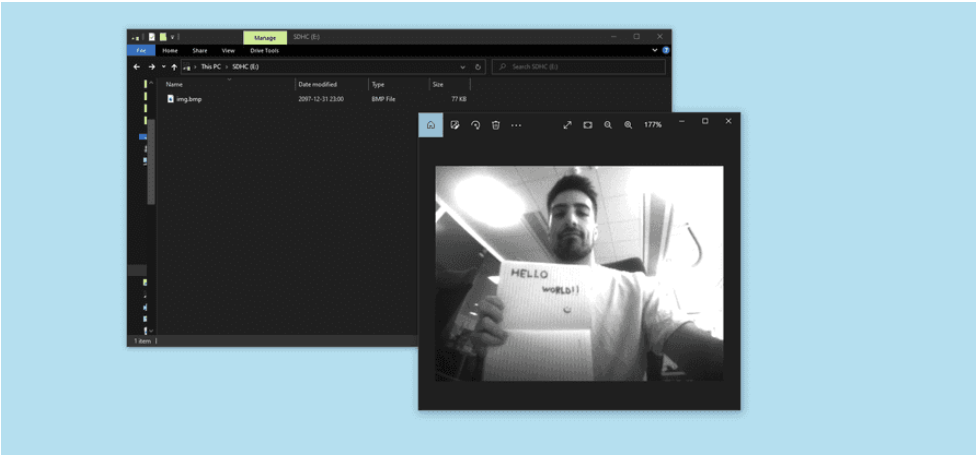
\includegraphics[width=0.7\linewidth]{Images/VisionShield/SavingImage.png}
		\caption{SavingImage}
		\label{SavingImage}
	\end{center}
\end{figure}

\textbf{Full Sketch}

{
	\captionof{code}{Simple sketch to save the image from vision shield}\label{SaveImage}
	\ArduinoExternal{}{../Code/Vision shield/SaveImage/SaveImage.ino}
}

\subsection{Conclusion}
In this example you learned how to capture frames with your Portenta Vision Shield's Camera in the Arduino IDE, encode it with the bitmap standards and save it to an SD Card and PC.









\section{Creating a Basic Face Filter With OpenMV}
In this example you will build a MicroPython application with OpenMV, to use the Portenta Vision Shield to detect faces and overlay them with a custom bitmap image. Think of it as building your own camera filter that puts a smile on every face it detects. This tutorial is based on the face detection example that comes with the OpenMV IDE. ~\ref{VisionShield} \cite{portentaFaceFilter:2024}

\subsection{Goals:}
\begin{itemize}
	\item How to use the OpenMV IDE to run MicroPython on Portenta
	\item How to use the built-in face detection algorithm of OpenMV
	\item Copying files to the internal Flash of the Portenta
	\item Using MicroPython to read files from the internal Flash \cite{portentaFaceFilter:2024}
\end{itemize}

\subsection{Required Hardware and Software:}
\begin{itemize}
	\item Portenta H7
	\item Portenta Vision Shield (LoRa or Ethernet)
	\item USB-C cable
	\item Arduino IDE 2.3+
	\item Portenta Bootloader Version 20+
	\item OpenMV IDE 2.6.4+ \cite{portentaFaceFilter:2024}
\end{itemize}

\subsection{The Haar Cascade Algorithm}
By harnessing the power of machine vision algorithms, objects can be detected in a camera stream. Those algorithms can be trained to detect the desired type of object. In this tutorial, you will use a machine learning based approach called Haar Cascade to detect faces.

\begin{figure}
	\begin{center}
		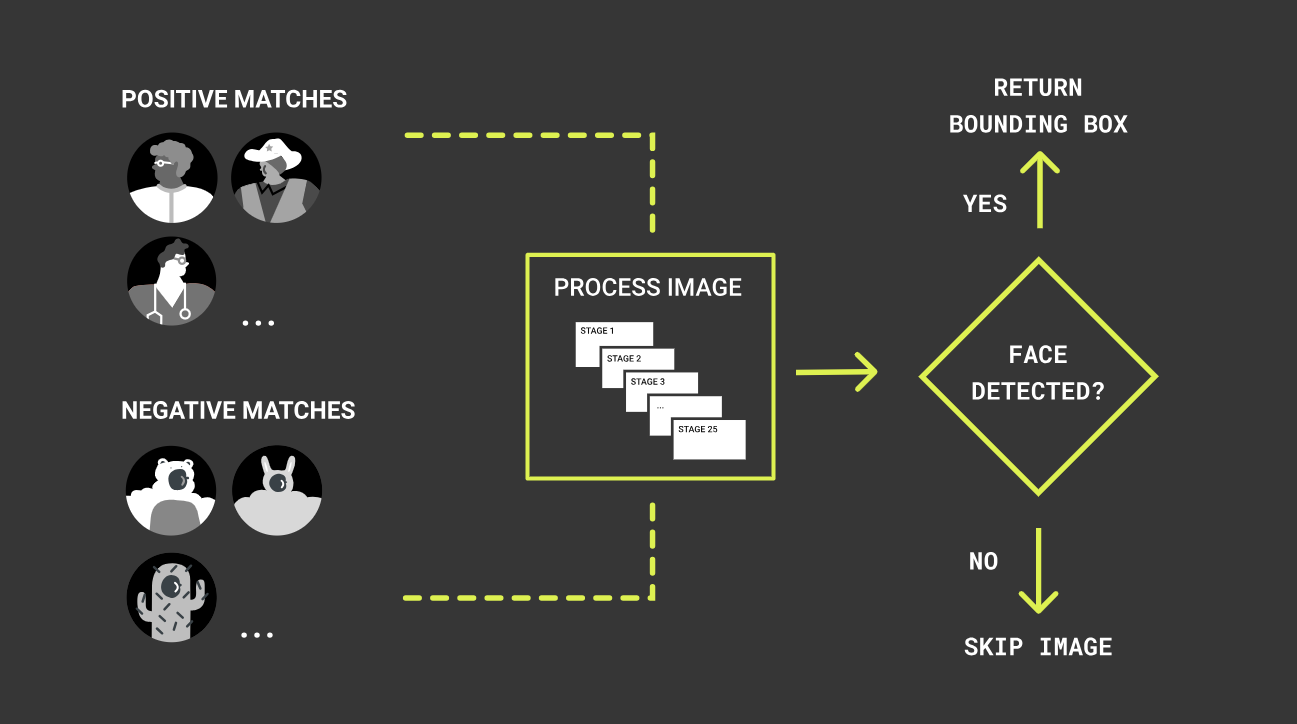
\includegraphics[width=0.7\linewidth]{Images/VisionShield/HaarCascade.png}
		\caption{HaarCascade}
		\label{HaarCascade}
	\end{center}
\end{figure}

This approach uses a cascade algorithm that has multiple stages, where the output from one stage acts as additional information for the next stage in the cascade. The different stages are responsible for detecting edges, lines, contrast checks and calculating pixel values in a given image. Larger areas of the image are checked first in the earlier stages, followed by more numerous and smaller area checks in later stages. The Haar Cascade function provided by OpenMV allows to specify the amount of stages. Fewer stages make the detection faster, while leading to more false positives.

The built-in Haar Cascade model for faces was trained with hundreds of images containing faces that are labeled as such and images that do not contain faces labeled differently. That allows the algorithm to distinguish such images after it is being trained.

\subsection{Instructions:}

\textbf{Creating the Face Detection Script}
For this tutorial, you will be using the OpenMV IDE along with the OpenMV firmware on your Portenta H7 to build the face detection script. If this is your first time using the Portenta Vision Shield and OpenMV, we recommend you to take a look at the "Configuring the Development Environment" section inside the Blob Detection tutorial to configure the development environment.

\subsubsection{The Basic Setup} Attach your Portenta Vision Shield to your Portenta H7 and open the OpenMV Editor. For this tutorial, you will create a new script that is based on the face detection example provided by OpenMV. Create a new script by clicking the "New File" button in the toolbar on the left side and save it as \SHELL{face detection.py}. \cite{portentaFaceFilter:2024}

\subsubsection{Importing the Modules} The script starts by importing the sensor, image and time modules for handling the camera sensor, using machine vision algorithms and time tracking functions. \SHELL{examples > Vision Shield to SD Card bmp > visionShieldBitmap.ino} 

First you need to include the needed libraries \cite{portentaFaceFilter:2024}

\begin{lstlisting}[language=C++, frame=single, numbers=left, basicstyle=\ttfamily\small]
	import sensor # Import the module for sensor related functions
	import image # Import module containing machine vision algorithms
	import time # Import module for tracking elapsed time
\end{lstlisting}

\subsubsection{Preparing the Sensor} The next step is to calibrate the camera sensor to achieve the best results using the sensor module. You can use the \SHELL{set contrast()} function to set the contrast of the sensor to its highest value (3). This can help the algorithm identifying lines and edges more easily. \SHELL{set gainceiling()} controls the amplification of the signal from the camera sensor including any associated background noise. For maximizing the detection success rate, it is recommended to set the camera frame size to HQVGA. \cite{portentaFaceFilter:2024}

\begin{lstlisting}[language=C++, frame=single, numbers=left, basicstyle=\ttfamily\small]
	# Sensor settings
	sensor.set_contrast(3)
	sensor.set_gainceiling(16)
	sensor.set_framesize(sensor.HQVGA)
	sensor.set_pixformat(sensor.GRAYSCALE)
\end{lstlisting}

\subsubsection{Displaying a Bitmap Image} Once you know the location of the faces in the camera image, you can overlay them with an image of your choice. OpenMV currently supports bmp, pgm or ppm image formats. Image formats with an alpha layer such as PNG are not supported yet.

In this tutorial you will use a preloaded smiley image in the monochrome Portable Bitmap Image (.pbm) format. This format consists of a matrix of zeroes and ones denoting black and white pixels. 1 stands for a black pixel, 0 for a white one. If you want to create your custom image, make sure you save it in one of the supported bitmap formats (bmp, pgm or ppm). You may use an image editor of your choice which supports exporting images in one of these formats. For this tutorial Adobe Photoshop was used.

Connect your Portenta board to your computer if you have not done so yet. Make sure you are running the OpenMV firmware on the Portenta. If you have not installed the OpenMV firmware yet, take a look at the "Configuring the Development Environment" section which explains how to proceed in that case.

Download this file containing the smiley bitmap and copy it to the Flash drive that was mounted when you connected the Portenta running the OpenMV firmware. \cite{portentaFaceFilter:2024}

\begin{figure}
	\begin{center}
		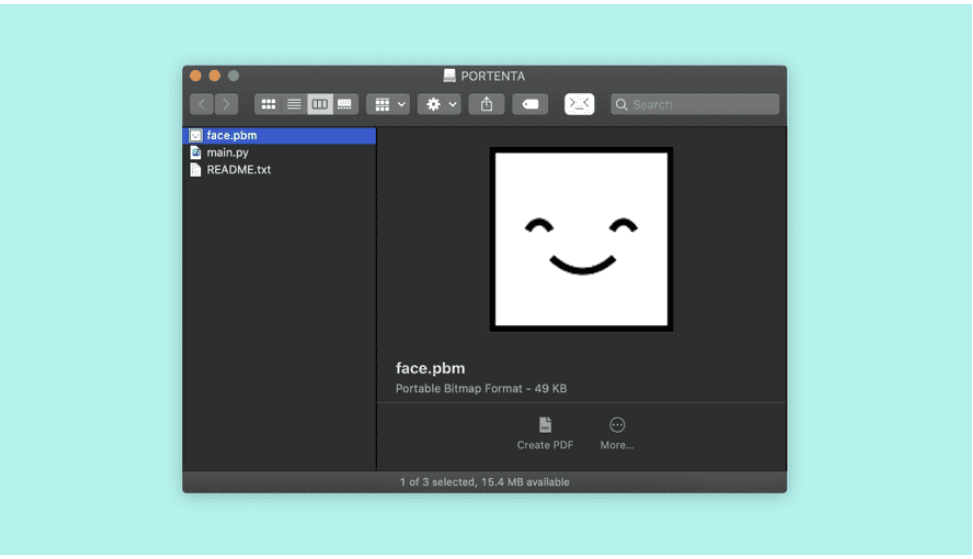
\includegraphics[width=0.7\linewidth]{Images/VisionShield/BitmapImage.png}
		\caption{BitmapImage}
		\label{BitmapImage}
	\end{center}
\end{figure}

Load the image into a variable called \SHELL{faceImage} using the \SHELL{Image()} function from the \SHELL{image} module. The initial slash refers to the root directory of the Flash drive. In order to use the image as an overlay to the camera stream, instead of directly displaying it, set the \SHELL{copy to fb} to False such that it does not get copied into the frame buffer automatically.

\begin{lstlisting}[language=C++, frame=single, numbers=left, basicstyle=\ttfamily\small]
	faceImage = image.Image("/face.pbm", copy_to_fb=False)
\end{lstlisting}

Before drawing the image on top of the camera stream you need to figure out the scale ratio to match the detected face size in the camera stream. The provided bitmap image comes in a 128x128 px resolution. You can calculate the correct scale ratio with the following formula:

\begin{lstlisting}[language=C++, frame=single, numbers=left, basicstyle=\ttfamily\small]
	faceX = boundingBox[0]
	faceY = boundingBox[1]
	faceWidth = boundingBox[2]
	
	# Calculates the scale ratio to scale the bitmap image to match the bounding box
	scale_ratio = faceWidth / faceImage.width()
\end{lstlisting}

You can then draw the scaled bitmap image on top of the camera image using the \SHELL{draw image} function:

\begin{lstlisting}[language=C++, frame=single, numbers=left, basicstyle=\ttfamily\small]
	# Draws the bitmap on top of the camera stream
	cameraImage.draw_image(faceImage, faceX, faceY, x_scale=scale_ratio, y_scale=scale_ratio)
\end{lstlisting}

\subsubsection{Uploading the Script} Let's program the Portenta with the complete script and test if the algorithm works. Copy the following script and paste it into the new script file that you created. \cite{portentaFaceFilter:2024}

{
	\captionof{code}{Simple sketch for bitmap image}\label{BitmapImage}
	\ArduinoExternal{}{../Code/Vision shield/Face Detection/face_detection.py}
}

Click on the "Play" button at the bottom of the left toolbar. Point the camera on the Portenta Vision Shield towards your face and check if the Portenta can detect it. Once it detects your face, it should be covered with a smiley.

\begin{figure}
	\begin{center}
		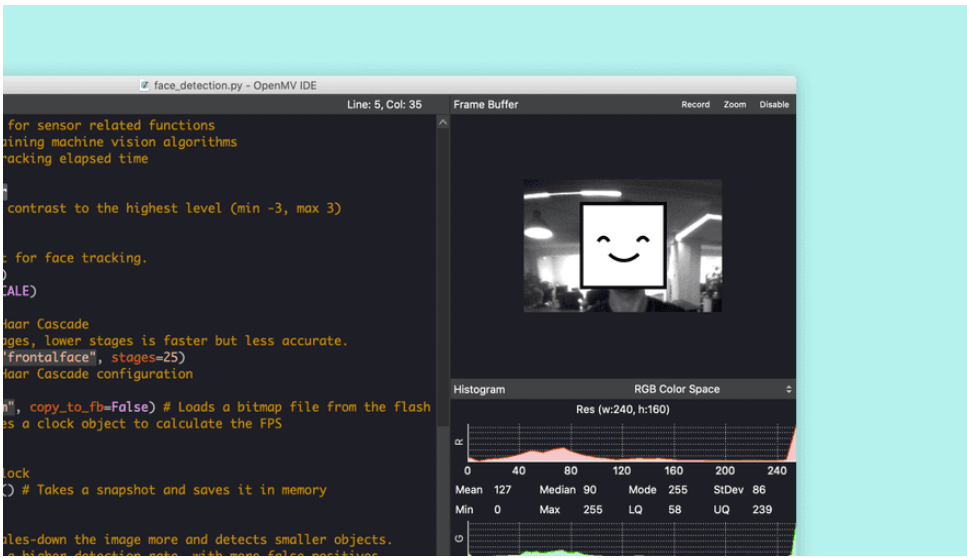
\includegraphics[width=0.7\linewidth]{Images/VisionShield/ImageOutput.png}
		\caption{ImageOutput}
		\label{ImageOutput}
	\end{center}
\end{figure}

\subsection{Conclusion}
In this example you learned how to use OpenMV's built-in face detection algorithm which is based on Haar Cascade. Furthermore, you learned how to copy a file to the internal flash and how to load an image from the Flash into the memory. You have also learned how to draw an image on top of a snapshot from the camera stream.
